\documentclass[preprint,12pt]{elsarticle}
\renewcommand*{\today}{March 29, 1686} % isso substitui a data de hoje para a escolhida

\usepackage{amssymb,amsmath,amsthm} %ferramentas matemáticas
\usepackage{hyperref} %links e referencias clicáveis
\hypersetup{pdfauthor=author} %para evitar alguns "warnings"
            
\usepackage[T1]{fontenc} %para enconding de letras com acentuação
% \usepackage{lineno}

\journal{Philosophi\ae\ Naturalis Principia Mathematica}

\begin{document}

\begin{frontmatter}

\title{Universal law of gravitation -- a simple \LaTeX\ example in the elsarticle class}

\author[1]{Sir Isaac Newton}

\author[2]{Robert Hooke}

\author[3]{Juan Manuel Costa Miscione\corref{cor1}}

\cortext[cor1]{corresponding author}
\ead{omanuelcosta@protonmail.com}

\affiliation[1]{organization={University of Cambridge},
            addressline={The Old Schools, Trinity Ln}, 
            city={Cambridge},
            postcode={325678}, 
            country={United Kingdom}}
            
\affiliation[2]{organization={Wadham College, University of Oxford},
            addressline={Parks Rd, Oxford OX1}, 
            city={Cambridge},
            postcode={928571}, 
            country={United Kingdom}}

\affiliation[3]{organization={Department of Metallurgical and Materials Engineering, Escola Polit\'ecnica da Universidade de S{\~a}o Paulo},
            addresline={Av. Prof. Mello Moraes, 2463,},
            postcode={5508-030},
            city={S\~ao Paulo},
            state={S\~ao Paulo},
            \country={Brazil},
            }

            
\begin{abstract}
This is our article on the newly discovered universal gravitation law, which is believed to define the movement of everything that exists, at all times, like planets (studied by Kepler and Galileo) and stuff. There is something wrong about the perihelion of Mercury, the red-shift of very far objects and the fact that the force is exerted by ``\emph{distance}''. But I'll let Einstein work that out in 221 years or so.
\end{abstract}

\begin{graphicalabstract}
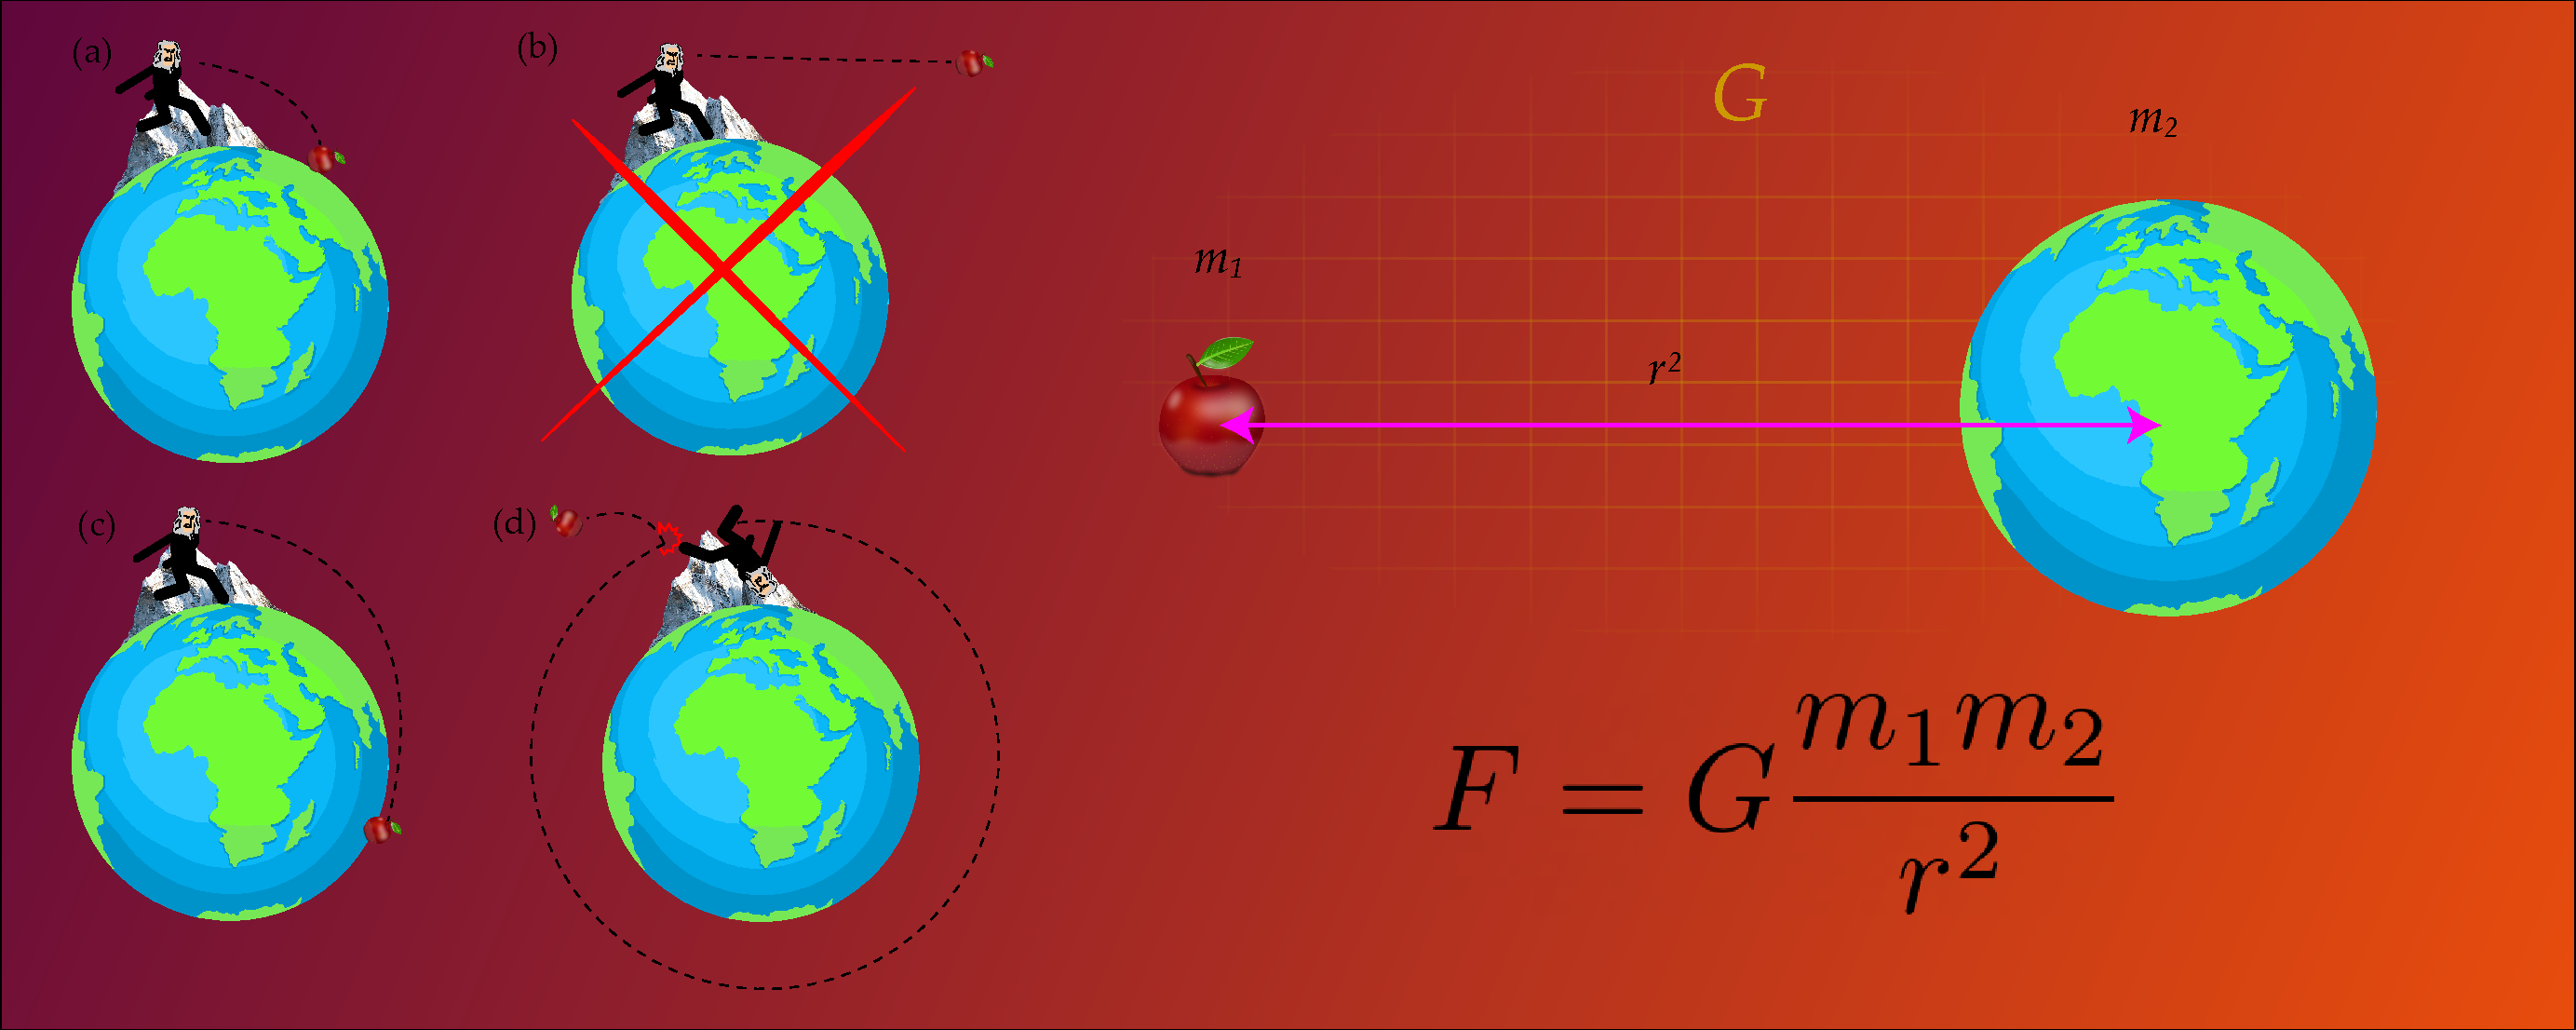
\includegraphics[width=\textwidth]{GA.pdf} %elsarticle já tem o pacote graphicx embutido
\end{graphicalabstract}

\begin{highlights}
\item We discovered gravity, yey!
\item It has to do with masses and distances between them
\item There is something wrong with Mercury's Perihelion
\item The fact that the forces are exerted by \emph{distance} is weird, too
\item Maybe Einstein will know the answer for these
\end{highlights}

\begin{keyword}
planets \sep forces \sep apples
\end{keyword}

\end{frontmatter}

% \linenumbers

\section{How does gravity work?}\label{s:introduction}
\label{sec:sample1}
So, imagine you have like an apple\footnote{I really like apples}, and you throw it really far away from the top of a 50 meters tall hill ($h=50$). According to some ancient Greek mathematician \cite{roller2010eratosthenes}, an arc describes the trajectory of the apple, just like shown in Figure \ref{fig:apple_throw}(a). Table \ref{tab:projectile} presents the trajectory of the apple if thrown at an horizontal speed of 50 m/s ($v_y=0$).

\begin{table}
    \centering
    \caption{Position of the apple when thrown from a hill with an initial horizontal speed of 50 m/s like in Figure \ref{fig:apple_throw}(a). The apple falls, independently, at a 9.8 m/s$^2$ acceleration.}
    \label{tab:projectile}
    \begin{tabular}{c c | r}
    \hline
    \multicolumn{2}{c}{position} & \\
    x [m] & y [m] & time [s] \\
    \hline
    0.0 & 50.0 & 0 \\
    25.0&48.8 & 0.5\\
    50.0&45.1 & 1.0 \\
    75.0&39.0 & 1.5 \\
    100.0&30.4 & 2.0 \\
    125.0&19.4 & 2.5 \\
    150.0&5.9 & 3.0 \\
    175.0&0 & 3.2 \\
    \hline
    \end{tabular}
\end{table}

The earth, as we already know, is round (even if there are still guys today who still don't believe it, IN 1686! -- can you imagine?), hence, the apple will fall on the Earth's surface. But what happens if we throw it, like, \emph{really}, \emph{really} far away, \emph{i.e.,} with very high speeds? Something interesting happens: the apple starts to curve around the Earth, falling farther and farther.

\begin{figure}[!ht]
    \centering
    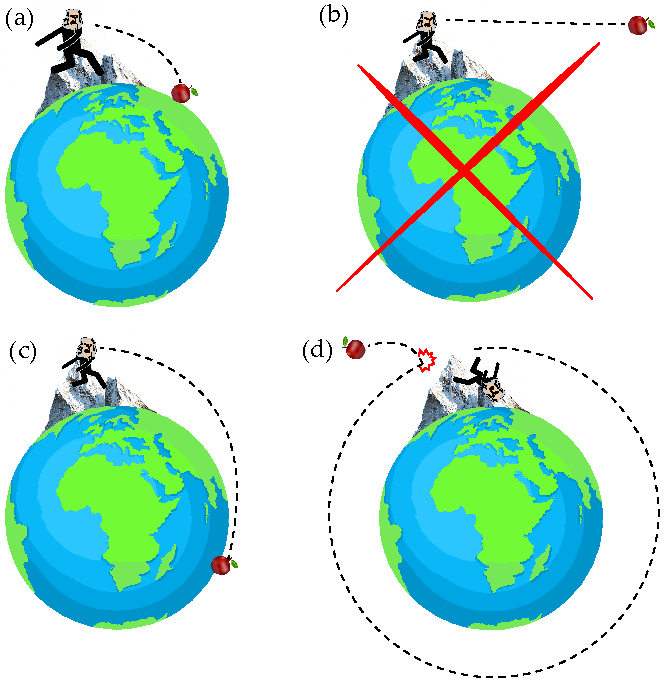
\includegraphics[width=0.85\textwidth]{figures/throwing_apple.pdf}
    \caption{Throwing an apple until it establishes an orbit around earth.}
    \label{fig:apple_throw}
\end{figure}

This is very interesting, because there is a certain speed on which the apple will actually start to \emph{orbit} around the globe... orbiting the globe like \emph{the moon}? or like the Earth around \emph{the Sun}? you can kinda see were I'm going right? As I said, there is no reason for why the apple should not just continue in straight line to eternity, as shown in Figure \ref{fig:apple_throw} (b), \emph{unless} there is a \emph{force} bringing it down. 

In a \emph{reduction ad absurdum}-kinda argument, what if the throw an object as heavy as the Sun? Well, then we will actually push the Earth rather than throw the Sun. Why? Well just imagine you are pushing a car... it's very heavy, but if you are strong, you can actually push yourself away from it --- because it is so much heavier than you. So, thinking about it, the Sun is heavy, and the Earth revolves around the Sun, and the moon is lighter, so it revolves around the Earth... it has something to do about the weight of both objects in orbit, right?

\section{Mathematical derivation -- kinda}\label{s:derivation}

Considering that the forces between the Earth and the Sun are the same, due to \emph{action and reaction}, we can say that the masses need to be included in our calculation, because only the Earth orbits the Sun, not the opposite. Also, the distance between them seems to be important: consider that mercury is very small, and very close to the Sun -- that means it's speed is lower, and, hence, its speed is way higher than, for example, a small planet but farther away from the Sun, like Mars. That means that the forces acting in Mercury may seem higher than with Mars, but also must be proportional to the distance between the bodies. Jupiter is heavier than both added together, so that the forces necessary to keep it rotating around the Sun are higher. BUT, it's orbit speed is just a little slower than Mars, but then again, Earth is a lighter than Jupiter, but closer to the Sun. So actually masses are important, too. This is confusing, did you get it?

Confused? fear no more, it all makes sense when you look at this very beautiful equation I came up with:

\begin{equation}\label{eqn:universal_law}
    F = G\frac{m_1 m_2}{r^2}
\end{equation}

This equations just summarized everything I failed to explain in the former paragraph! The forces are dependent on the product of the mass of both bodies ($m_1$ and $m_2$) divided by the squared distance between the center of both masses ($r^2$). The $G$ is a constant that must exist in order for this equation to actually work. So I guess I cannot leave you with that. Ok, I'll try to find that constant. While I do it check out Figure \ref{fig:illustration}, that illustrates the masses and distance presented in Equation \ref{eqn:universal_law}.

\begin{figure}
    \centering
    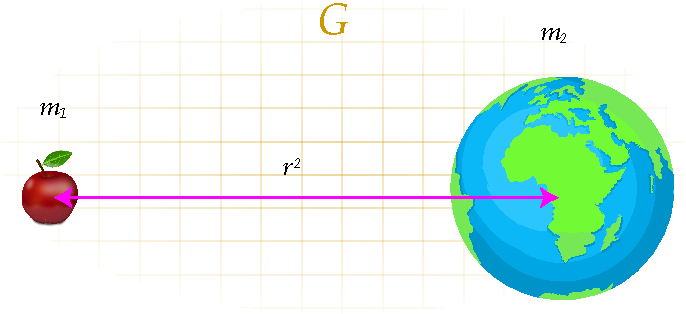
\includegraphics{figures/scheme.pdf}
    \caption{Illustration of the units presented in the universal law of gravitation.}
    \label{fig:illustration}
\end{figure}

Some Italian Jesuits \cite{zubov2008physical,riccioliastronomiae} discovered that stuff in earth falls with the square of the time. Interestingly enough, the accelerations of object follow a constant 9.8 m/s$^2$, that is 9.8 meters per second per second! just like I showed you in Table \ref{tab:projectile}. From my law of motion:

\begin{equation}
F = m a
\end{equation}

\noindent
if we are talking about acceleration of gravity we might just call $a\rightarrow g$, and $m$ is the mass of the object that suffers acceleration from Earth (which happens to be the $m_1$ in Equation) \ref{eqn:universal_law}

\begin{equation}\label{eqn:law_motion_g}
F = m_1 g 
\end{equation}

\noindent
if we substitute $F$ in Equation \ref{eqn:law_motion_g} with Equation \ref{eqn:universal_law}, we get:

\begin{equation}
m_1 g = G\frac{m_1 m_2}{r^2}
\end{equation}

\noindent
simplifying we get:

\begin{equation}
    g = G \frac{m_2}{r^2}
\end{equation}
\noindent
with $r^2$ being the radius of the Earth, which we know from the works of our old Greek mathematician \cite{roller2010eratosthenes}, which is $6.4\times10^6$ m. This means that the acceleration of the Earth is just dependent on the mass of the Earth, which is $m_2$. This is kinda of a problem, because we don't actually know that... how heavy is the Earth?. That's why I, Sir Isaac Newton, never determined the gravitational constant myself, but a scientist nearly 100 years later than me. So I'm going to cheat by Googling it: I know that the Earth of the mass is $6\times 10^24$ kg \cite{clotfelter1987cavendish}. That means:

\begin{align} %\usepackage{amsmath} provides the \begin{align} environment
    9.8 =\quad & G \frac{6\times 10^{24}}{(6.4\times10^6)^2} \\
    G =\quad & \frac{9.8(6.4\times10^6)^2)}{6\times 10^{24}}\\
    G =\quad & 6.7\times10^{-11}
\end{align} %quad add spaces between things in math mode

\noindent
which is close enough to the universal gravitational constant in the SI.

\section{Conclusion}

So we concluded that gravity exists, it's real, and it has the properties described in this article in Sections \ref{s:introduction} and \ref{s:derivation}. There is also some more info on this in \ref{s:appendix}.

Congratulations, now nothing is floating around randomly anymore, as I've invented gravity. Haha! I know, it didn't change anything...

\noindent
...or did it?

<<<<<<< HEAD
\bibliographystyle{elsarticle-num} %o elsarticle utiliza o pacote bibtex em vez do biblatex -- os comandos são \bibliographystyle e \bibliography para adicionar o .bib
\bibliography{refs.bib}
=======
 \bibliographystyle{elsarticle-num} %o elsarticle utiliza o pacote bibtex em vez do biblatex -- os comandos são \bibliographystyle e \bibliography para adicionar o .bib
 \bibliography{refs.bib}
>>>>>>> 20ae0a6b42f26e0d211b26a9c94ab001be4a5cb3

\newpage
\appendix
\section{One simple Appendix}\label{s:appendix}

There is actually no more info here: it was just a prank, bro.

\end{document}